% !TEX root = ../../../main.tex
% 来源：中学数学实验教材·第三册（高中数学）
% 章节：直线、平面坐标化 / 直线坐标化
% 原始文件：2.tex，行 75-87
% 类型：tikz
% ---
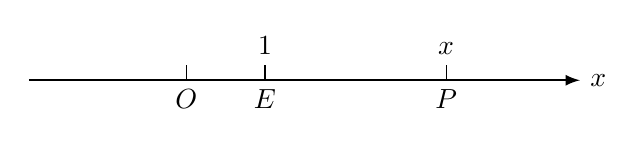
\begin{tikzpicture}[>=latex]
\draw[thick, ->] (-2,0)--(5,0)node[right]{$x$};
\foreach \x in {0,1,3.3}
{
    \draw(\x,0)--(\x,0.2);
}
\node at (0,0) [below]{$O$};
\node at (1,0) [below]{$E$};
\node at (3.3,0) [below]{$P$};
\node at (1,0.2) [above]{$1$};
\node at (3.3,0.2) [above]{$x$};

\end{tikzpicture}
